\section{\textit{Embeddings}}

El primer enfoque que se le dio a este problema de clasificación consistió en construir los \textit{embeddings} (representaciones vectoriales de las palabras) con un modelo de Word2Vec. Este modelo utiliza una red neuronal para aprender las asociaciones de palabras a partir de un corpus de documentos o sentencias. \\

Para esto se utilizó la implementación de Word2Vec de la librería de \texttt{gensim}. A continuación se explican algunos de los parámetros clave del modelo y los valores que se definieron para los mismos para este trabajo:

\begin{itemize}
    \item Tamaño del Embedding (\textit{embedding\_size}): La dimensionalidad del vector resultante como represesntación de cada uno de los términos. Se decidió tratar con 3 tipos de tamaños: pequeño (dim=15), mediano (dim=75) y grande (dim=150).
    
    \item Window: Ventana de tamaño que utiliza el modelo para considerar las palabras similares entre sí. En este caso se experimento con varios tamaños desde 1 hasta 10 y los mejores resultados se obtuvieron entre 2 y 3. Es decir, el modelo considera 2-3 palabras antes y despues de la palabra en cuestión como palabras similares.
    
    \item Min Count: Frecuencia mínima que debe tener una palabra para considerarla dentro del modelo, esto elimina términos extraños y muy poco frecuentes. Se definió en 10, lo que redujo considerablemente el tamaño del vocabulario.
    
    \item SG: Si utilizar un modelo de \textit{skipgram} o \textit{cbow}. 
    
    \item Negative: El número de palabras utilizado como ejemplo negativo al momento de entrenar el modelo. 
\end{itemize}

\subsection{2D Plots}

Dado el tamaño de los \textit{embeddings} (15, 75 y 150), se utiliza una técnica de reducción de dimensionalidad para poder visualizar algunos de los términos (vectores) interesantes y sus relaciones en un plano 2D. En este caso, se decidió utilizar la técnica de Análisis de Componentes Principales (o PCA por sus siglas en inglés). Esta técnica...

\subsubsection{Simpsons Dataset}

\begin{figure}[H]

\centering
\begin{minipage}{0.47\textwidth}
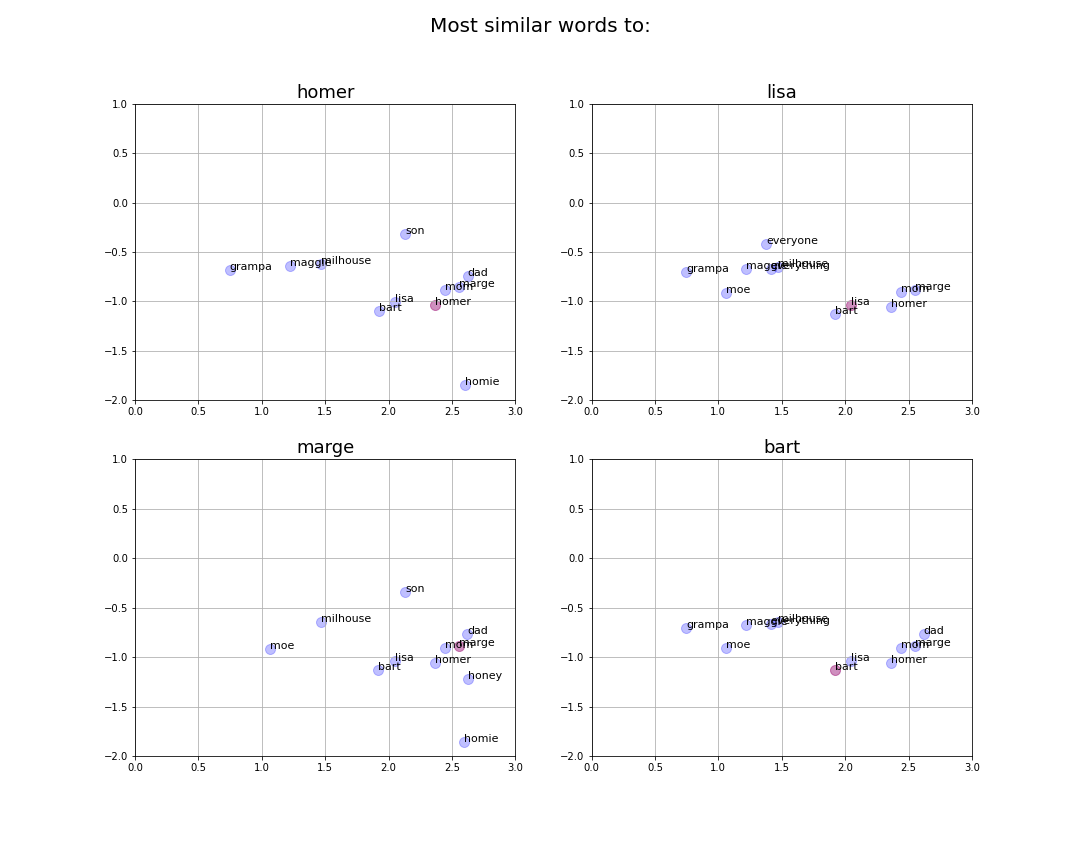
\includegraphics[trim=4.2cm 3cm 3.7cm 2.7cm, clip=true, width=\textwidth]{results/embeddings/simpsons_similar_15.png}
\caption*{a) DIM = 15}
\end{minipage}\hfill
\begin{minipage}{0.47\textwidth}
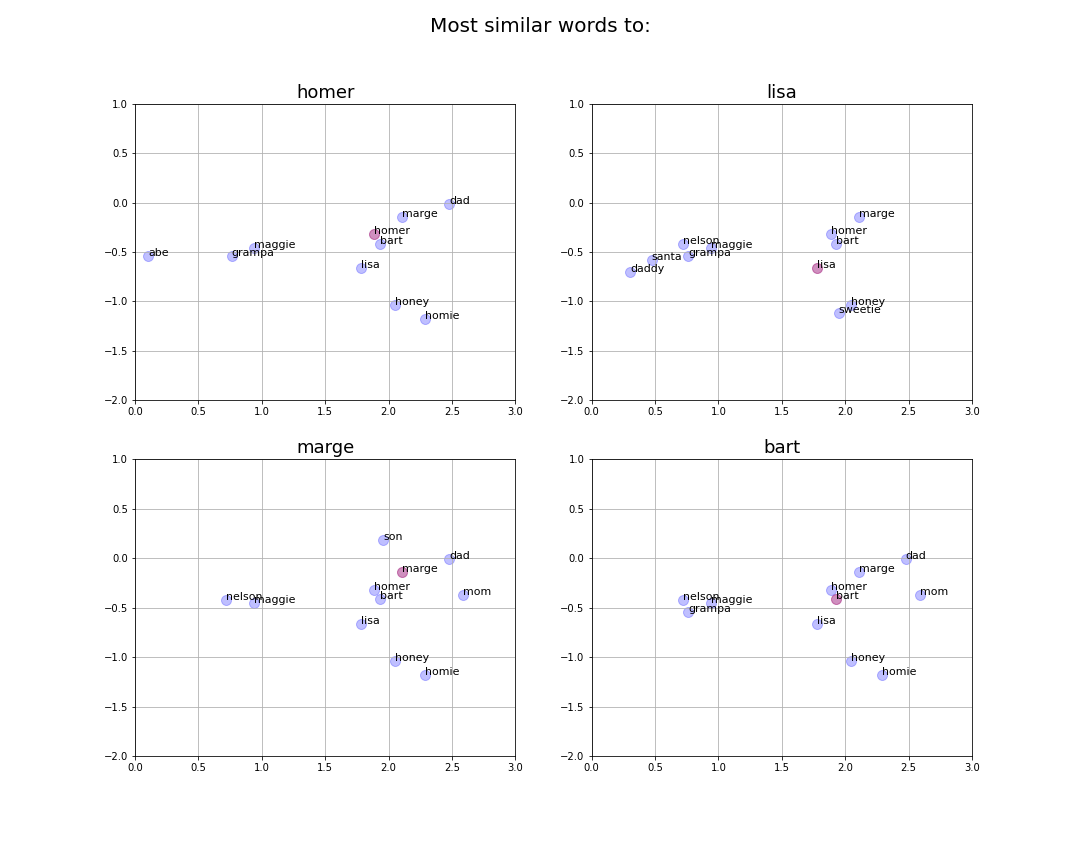
\includegraphics[trim=4.2cm 3cm 3.7cm 2.7cm, clip=true, width=\textwidth]{results/embeddings/simpsons_similar_75.png}
\caption*{b) DIM = 75}
\end{minipage}\par
\vskip\floatsep% normal separation between figures
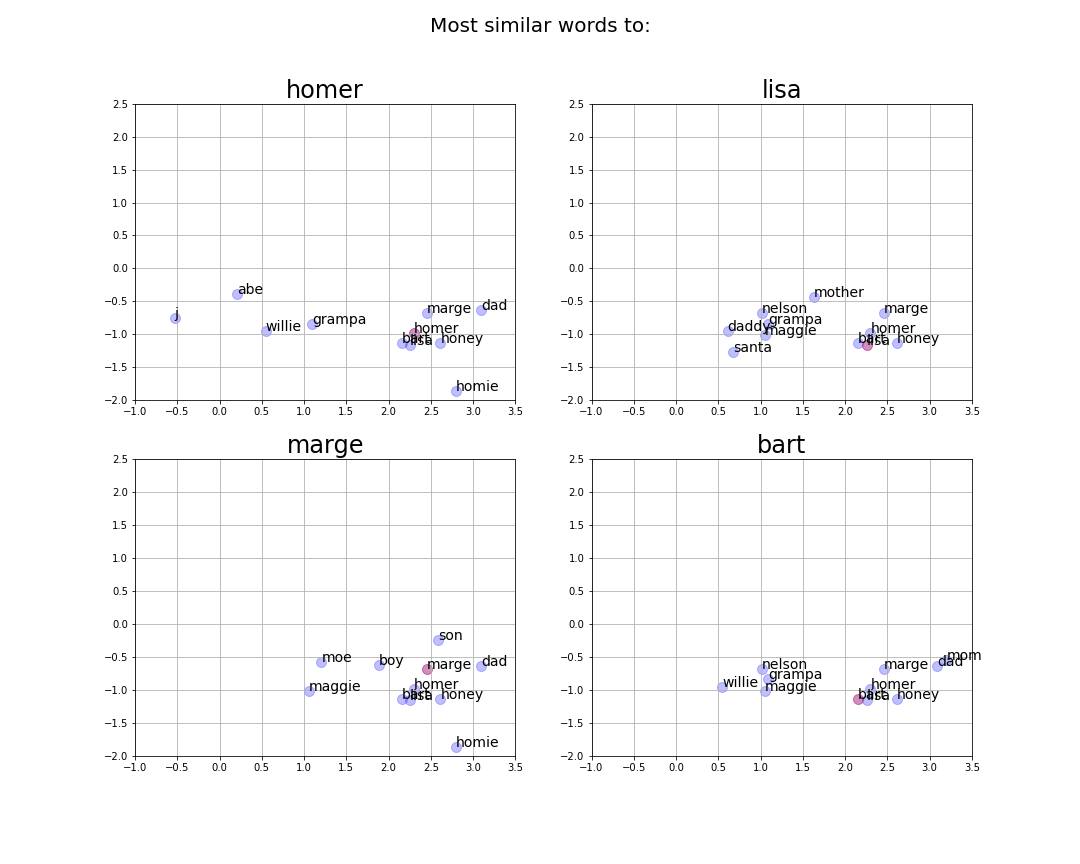
\includegraphics[trim=4.2cm 3cm 3.7cm 2.7cm, clip=true, width=0.45\textwidth]{results/embeddings/simpsons_similar_150.png}
\caption*{c) DIM = 150}
\caption{\textit{Embeddings} de los personajes principales de los \textbf{\textit{Simpsons}} y los términos más similares proyectados en un plano 2D para distintos tamaño de \textit{embedding}}
\label{fig:simpsons_sim_words}

\end{figure}


\subsubsection{Friends Dataset}

\begin{figure}[H]

\centering
\begin{minipage}{0.47\textwidth}
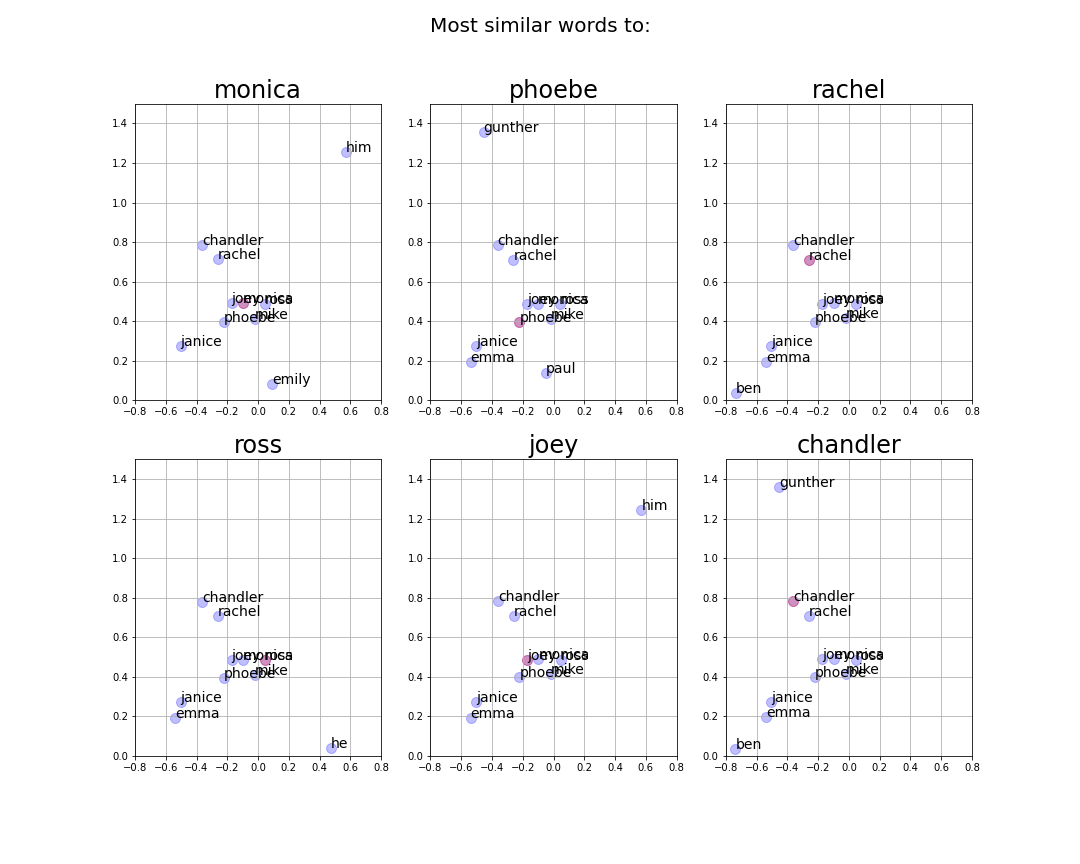
\includegraphics[trim=4.2cm 3cm 3.7cm 2.7cm, clip=true, width=\textwidth]{results/embeddings/friends_similar_15.png}
\caption*{a) DIM = 15}
\end{minipage}\hfill
\begin{minipage}{0.47\textwidth}
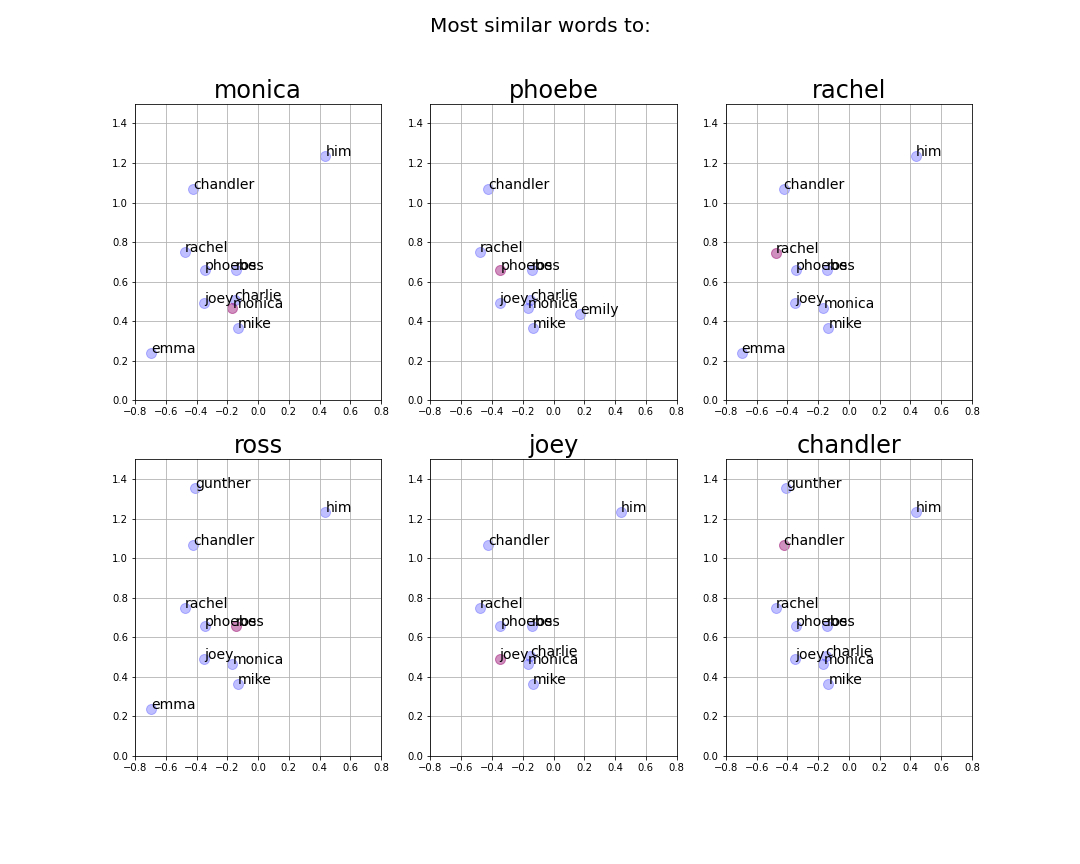
\includegraphics[trim=4.2cm 3cm 3.7cm 2.7cm, clip=true, width=\textwidth]{results/embeddings/friends_similar_75.png}
\caption*{b) DIM = 75}
\end{minipage}\par
\vskip\floatsep% normal separation between figures
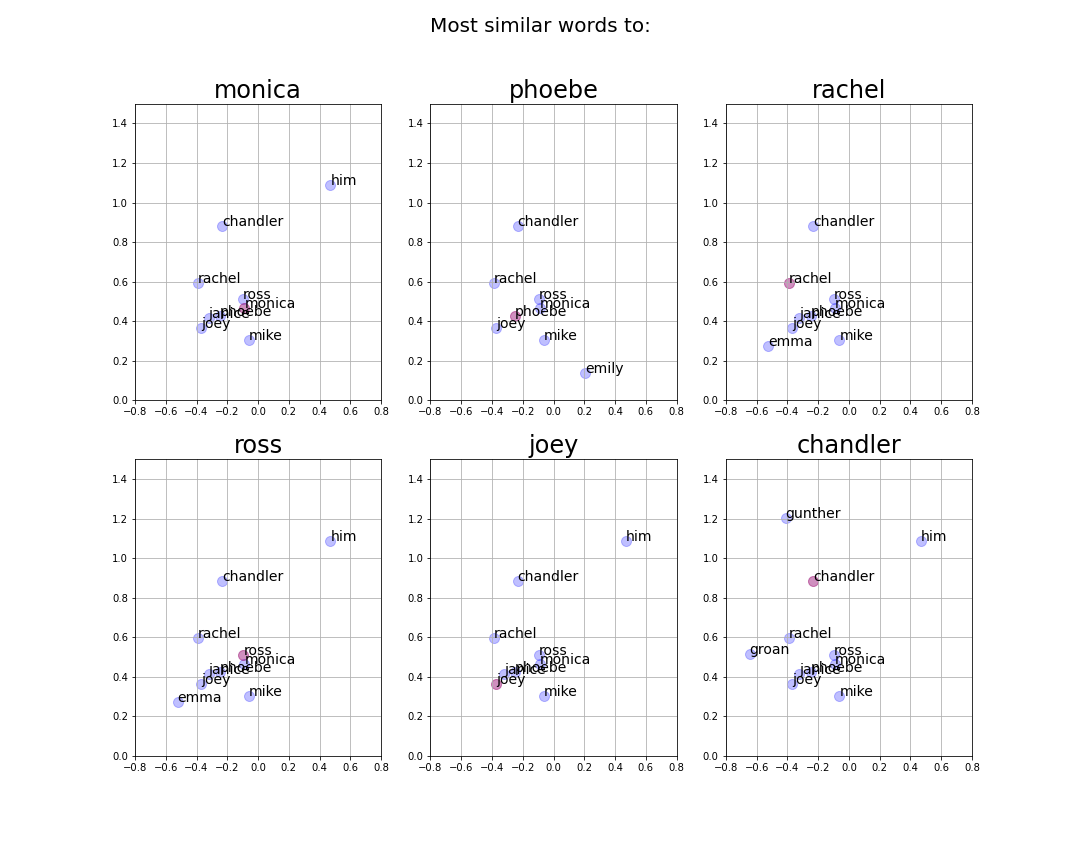
\includegraphics[trim=4.2cm 3cm 3.7cm 2.7cm, clip=true, width=0.45\textwidth]{results/embeddings/friends_similar_150.png}
\caption*{c) DIM = 150}
\caption{\textit{Embeddings} de los personajes principales de \textbf{\textit{Friends}} y los términos más similares proyectados en un plano 2D para distintos tamaño de embedding}
\label{fig:friends_sim_words}

\end{figure}

\subsection{Relaciones interesantes}

Finalmente, una de características principales y bastante interesantes de los \textit{embeddings} es que logran capturar la relación semántica de las palabras en un espacio vectorial. Razón por la cual los términos se pueden operar y se pueden encontrar algunas relaciones bastante interesantes. A partir de los modelos de word2vec construidos en esta sección se indagaron en algunas de las relaciones que surgieron en tres niveles diferentes:

\begin{itemize}
    \item \textbf{Similaridad:} ¿Qué tan similares eran dos palabras?
    
    \item \textbf{Analogía:} ¿Qué palabra $w_x$ es a $w_3$ como $w_1$ es a la palabra $w_2$?
    
    \item \textbf{Coincidencia (\textit{doesn't match}):} ¿Cuál de las palabras o términos es el menos similar entre estos?
\end{itemize}

\subsubsection{Simpsons Dataset}

\begin{figure}[H]
    \centering
    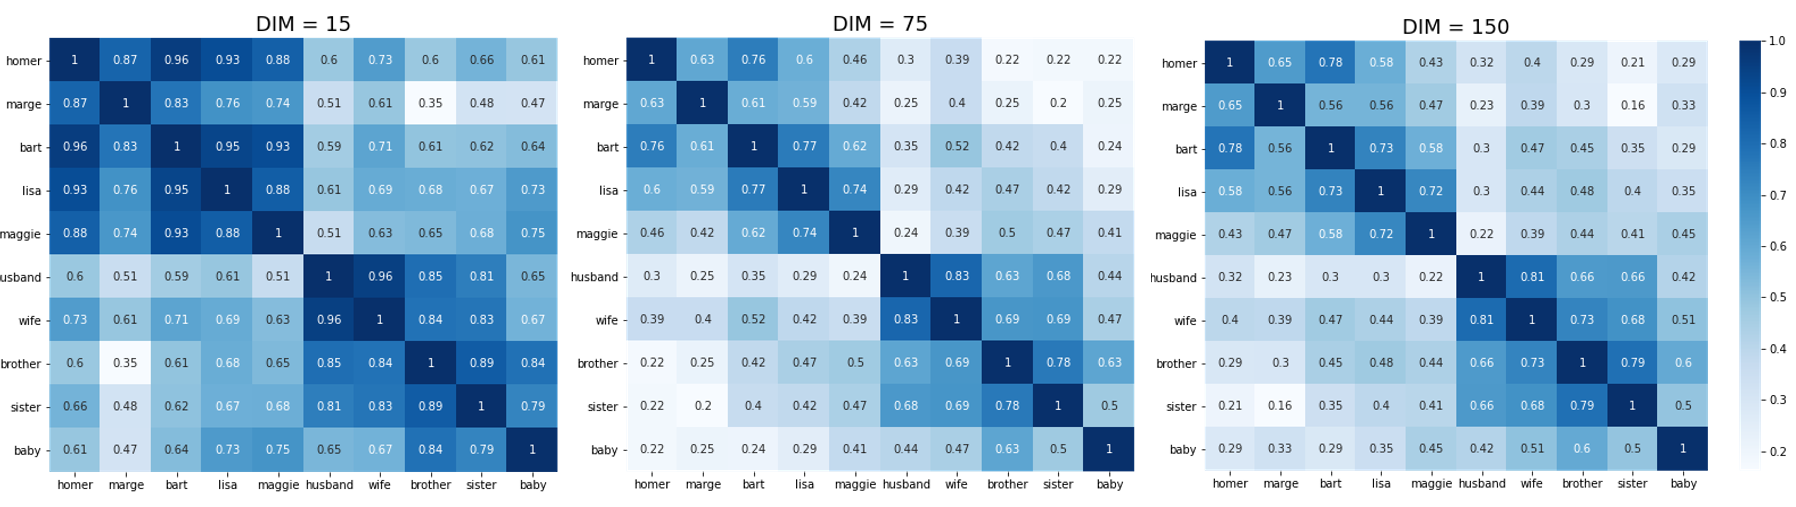
\includegraphics[width=\textwidth]{doc/images/simpsons_sim_matrix.png}
    \caption{Caption}
    \label{fig:simpsons_sim_matrix}
\end{figure}

\subsubsection{Friends Dataset}

\begin{figure}[H]
    \centering
    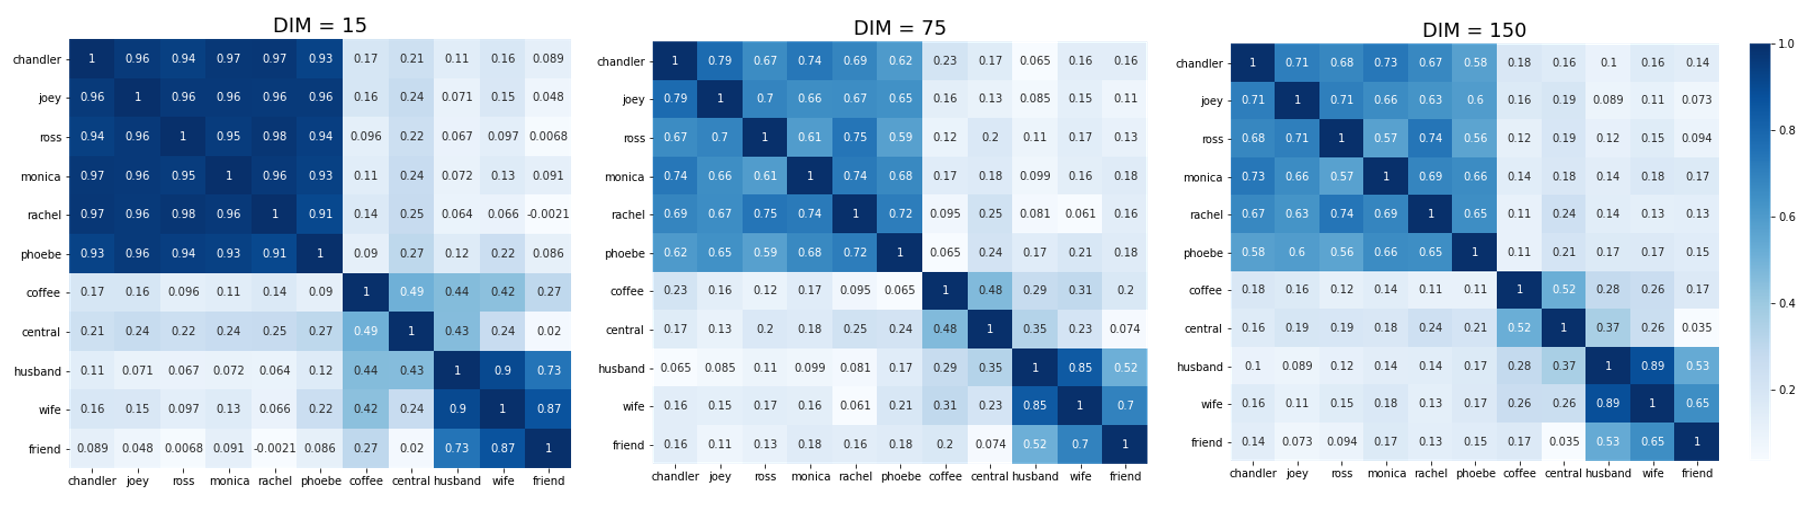
\includegraphics[width=\textwidth]{doc/images/friends_sim_matrix.png}
    \caption{Caption}
    \label{fig:friends_sim_matrix}
\end{figure}

\newpage